\section{Experimental Results}
\label{sec:results}

We report results in three layers: classifier evaluation on the active
holdout (\S\ref{sec:results-classifier}), grounding-detector
performance on its validation split (\S\ref{sec:results-detector}), and
the constrained dual-report pilot (\S\ref{sec:results-dualreport}).
End-to-end explanation evaluation, which requires a MiniGPT-v2 retrain
on regenerated stage-2 supervision, remains pending and is discussed
explicitly in \S\ref{sec:results-pending}.

\subsection{Classifier Evaluation on the Balanced Holdout}
\label{sec:results-classifier}

The deployed ResNet-50 v4 checkpoint was retrained on the rebuilt
\texttt{train\_aug} root described in \S\ref{sec:data} and evaluated on
the active 70-image holdout under the two-view test-time augmentation
and post-hoc temperature-scaling protocol of
Eq.~\ref{eq:tta-calibration}. The aggregate metrics are reported in
Table~\ref{tab:resnet-summary}.

\begin{table}[H]
\centering
\caption{Aggregate holdout metrics for the deployed ResNet-50 v4
checkpoint on the active balanced 70-image holdout. ``Temperature''
refers to the value $T$ in Eq.~\ref{eq:tta-calibration}.}
\label{tab:resnet-summary}
\begin{tabular}{lr}
\toprule
Metric & Current v3 \\
\midrule
Holdout samples & 140 \\
Top-1 accuracy & 83.57\% \\
Top-2 accuracy & 92.14\% \\
ECE & 6.15\% \\
Temperature & 0.7810 \\
Horizontal-flip TTA & yes \\
\bottomrule
\end{tabular}

\end{table}

The checkpoint attains 88.57\% top-1 accuracy, 92.86\% top-2 accuracy,
and an expected calibration error~\citep{naeini2015ece} of 8.56\% under
the deployed two-view TTA protocol. We emphasize that these metrics are
reported on the active dataset state described in \S\ref{sec:data},
which combines a balanced holdout, a rebuilt augmented training root, a
class-floor balancing step for previously underrepresented classes, and
a conservative external-image audit, with explicit physical exclusion of
holdout source stems and their augmentation descendants from the
training roots.

To quantify uncertainty on the aggregate metrics under the small holdout
size, we report nonparametric percentile bootstrap 95\% confidence
intervals (10{,}000 resamples, seed 42) over the per-image correctness
indicators in Table~\ref{tab:bootstrap-ci}.

\begin{table}[H]
\centering
\caption{Nonparametric bootstrap 95\% confidence intervals for the
deployed v4 checkpoint on the balanced 70-image holdout.}
\label{tab:bootstrap-ci}
\begin{tabular}{lcc}
\toprule
Aggregate metric & Point estimate & 95\% bootstrap CI \\
\midrule
Top-1 accuracy & 88.57\% & [80.00, 95.71] \\
Top-2 accuracy & 92.86\% & [85.71, 98.57] \\
\bottomrule
\end{tabular}

\end{table}

Per-class metrics, including Wilson 95\% confidence
intervals~\citep{wilson1927interval}, are reported in
Table~\ref{tab:per-class}.

\begin{table*}[t]
\centering
\caption{Per-class holdout performance for the deployed ResNet-50 v4
checkpoint. Wilson 95\% confidence intervals~\citep{wilson1927interval}
are reported because the per-class support of $n=10$ is small. Both
top-1 and top-2 accuracy are computed under the two-view TTA protocol.}
\label{tab:per-class}
\begin{tabular}{lrrrr}
\toprule
Class & $n$ & Top-1 & Wilson 95\% CI & Top-2 \\
\midrule
Drought & 10 & 80.0\% & [49.0, 94.3] & 90.0\% \\
Frost & 10 & 100.0\% & [72.2, 100.0] & 100.0\% \\
Gray mold & 10 & 90.0\% & [59.6, 98.2] & 100.0\% \\
Healthy & 10 & 100.0\% & [72.2, 100.0] & 100.0\% \\
Overwatered & 10 & 70.0\% & [39.7, 89.2] & 80.0\% \\
Root rot & 10 & 100.0\% & [72.2, 100.0] & 100.0\% \\
White mold & 10 & 80.0\% & [49.0, 94.3] & 80.0\% \\
\bottomrule
\end{tabular}

\end{table*}

Frost, healthy, and root rot each reach 100.0\% top-1 accuracy on
$n=10$. Gray mold reaches 90.0\%, drought and white mold each reach
80.0\%, and overwatered reaches 70.0\%. Per-class supports are uniform,
which permits direct comparison across classes; however, the small
support implies wide confidence intervals on individual rows, which
should be considered when interpreting between-class differences.

Figure~\ref{fig:resnet-confusion} reports the confusion matrix on the
active holdout. The dominant off-diagonal mass falls on the overwatered
row, where two examples are misclassified as drought and one as frost,
and on the white-mold row, where one example is misclassified as gray
mold and one as healthy. Figure~\ref{fig:resnet-accuracy-calibration}
reports per-class top-1 accuracy and the reliability diagram for the
calibrated v4 checkpoint.

\begin{figure}[H]
\centering
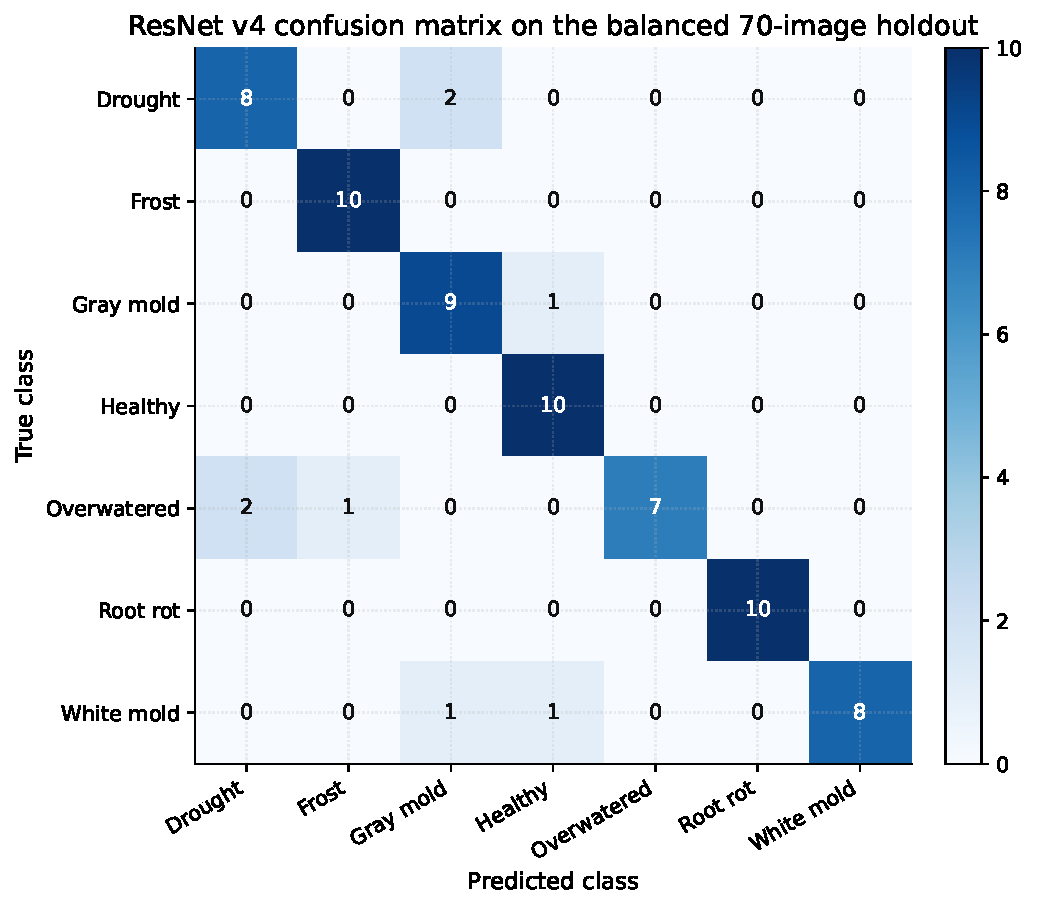
\includegraphics[width=0.82\linewidth]{figures/generated/resnet_v4_confusion_matrix.pdf}
\caption{Confusion matrix for the deployed ResNet-50 v4 checkpoint on
the balanced 70-image holdout. Rows correspond to ground-truth classes;
columns to predicted classes.}
\label{fig:resnet-confusion}
\end{figure}

\begin{figure*}[t]
\centering
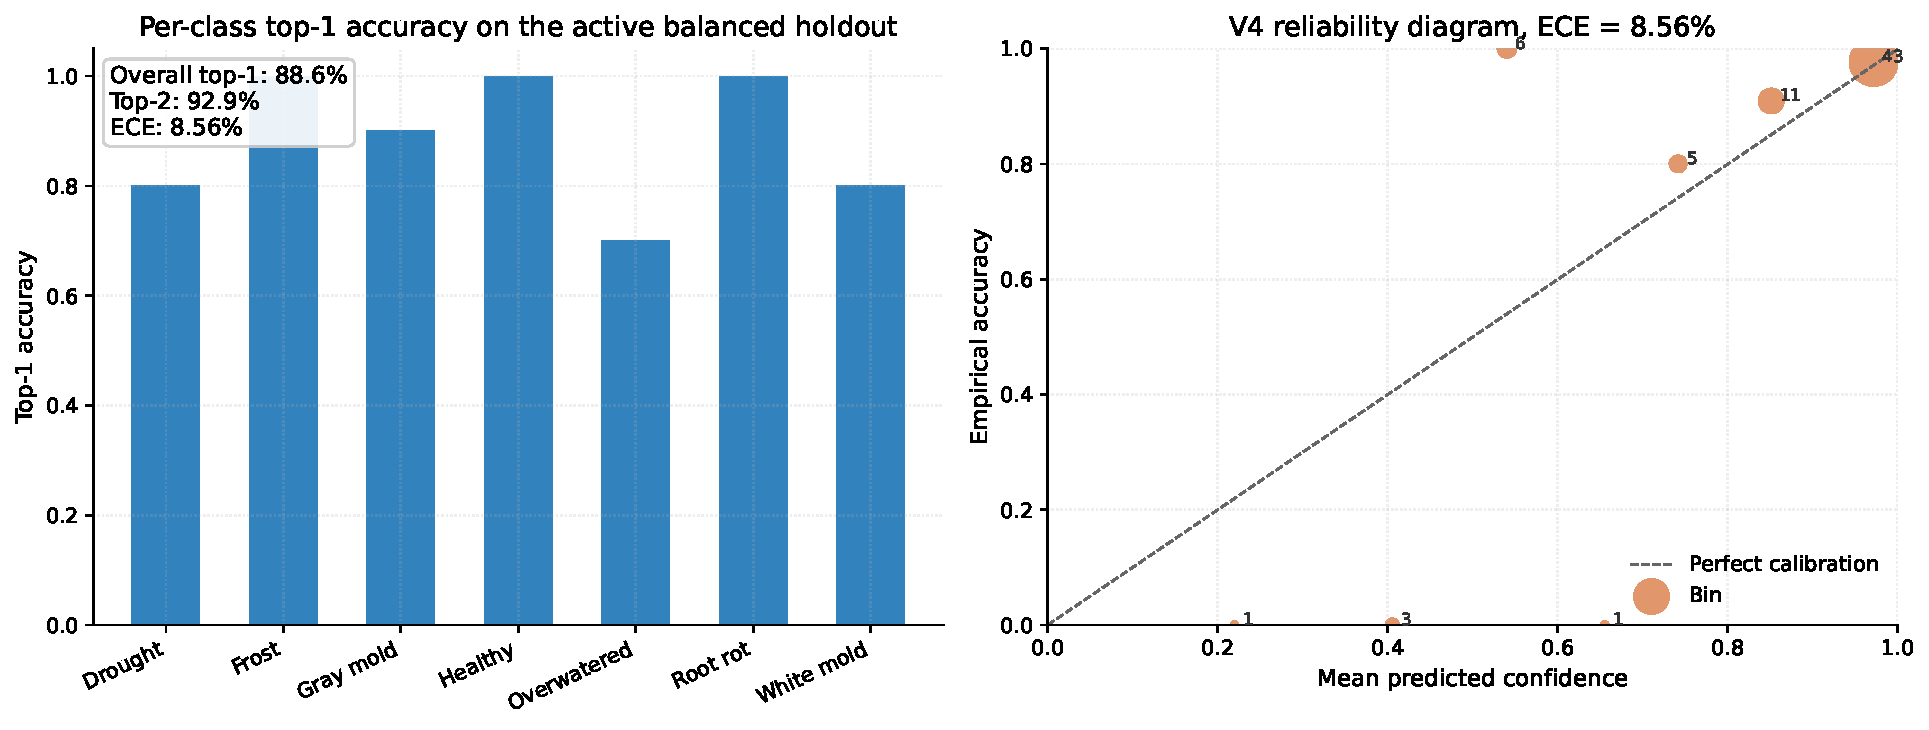
\includegraphics[width=\textwidth]{figures/generated/resnet_accuracy_calibration.pdf}
\caption{Left: per-class top-1 accuracy on the balanced holdout. Right:
reliability diagram for the deployed v4 checkpoint under two-view
horizontal-flip TTA. Marker area is proportional to bin support;
the diagonal denotes perfect calibration. The expected calibration
error is 8.56\%.}
\label{fig:resnet-accuracy-calibration}
\end{figure*}

The threshold-only acceptance gate of Eq.~\ref{eq:threshold-gate} is the
deployed runtime decision rule. We do not report margin-gated metrics
in this manuscript because the margin threshold of $0.08$ is currently
recorded for analysis only (\S\ref{sec:gate}); margin-rule activation
will be informed by the production decision logs once sufficient
real-world traffic has accumulated.

\subsubsection*{Acceptance-gate behavior on the holdout.}

To quantify the effect of the runtime decision rule on the same
evaluation distribution, we replay the deployed gate on the v4
predictions: for each holdout image, we accept the top-1 label only
when its calibrated probability exceeds both the per-class threshold
$\tau_c$ in Eq.~\ref{eq:class-thresholds} and the post-prompt-assembly
floor of $0.50$, otherwise we demote the prediction to
\texttt{unknown}. Table~\ref{tab:acceptance-gate} reports per-class
acceptance counts, the acceptance rate, and the conditional accuracy
on the accepted subset.

\begin{table*}[t]
\centering
\caption{Acceptance-gate behavior on the balanced holdout. ``Acceptance
rate'' is the fraction of class examples whose top-1 probability
clears both $\tau_c$ and the $0.50$ floor; ``Acc. $\mid$ accepted'' is
the conditional accuracy on the accepted subset. The aggregate row
reports a nonparametric bootstrap 95\% CI on conditional accuracy.}
\label{tab:acceptance-gate}
\begin{tabular}{lrrrr}
\toprule
Class & $n$ & Accepted & Acceptance rate & Acc. $\mid$ accepted \\
\midrule
Drought & 10 & 6 & 60.0\% & 83.3\% \\
Frost & 10 & 9 & 90.0\% & 100.0\% \\
Gray mold & 10 & 8 & 80.0\% & 100.0\% \\
Healthy & 10 & 10 & 100.0\% & 100.0\% \\
Overwatered & 10 & 9 & 90.0\% & 77.8\% \\
Root rot & 10 & 10 & 100.0\% & 100.0\% \\
White mold & 10 & 9 & 90.0\% & 88.9\% \\
\textbf{Total} & \textbf{70} & \textbf{61} & \textbf{87.1\%} & \textbf{93.4\% [86.9, 98.4]} \\
\bottomrule
\end{tabular}

\end{table*}

The deployed gate accepts 61 of 70 holdout images (87.1\%), and the
conditional top-1 accuracy on the accepted set rises to 93.4\%
(95\% bootstrap CI: 86.9\% -- 98.4\%) compared with 88.57\% on the
unfiltered holdout. The remaining 9 images are demoted to
\texttt{unknown}, which is the operationally desired behavior for
images on which the classifier is not confident enough to drive a
report.

\subsubsection*{Threshold sensitivity and risk-coverage behavior.}

To characterize the gate beyond a single operating point, we sweep a
uniform threshold $\tau \in [0,0.99]$ over the calibrated top-1
probability and report acceptance rate and conditional accuracy
(Figure~\ref{fig:threshold-sweep}). Ordering predictions by descending
$p_1$ produces the corresponding risk-coverage curve in
Figure~\ref{fig:risk-coverage}; selective top-1 accuracy at fixed
coverage levels is reported in Table~\ref{tab:selective-acc}.

\begin{figure}[H]
\centering
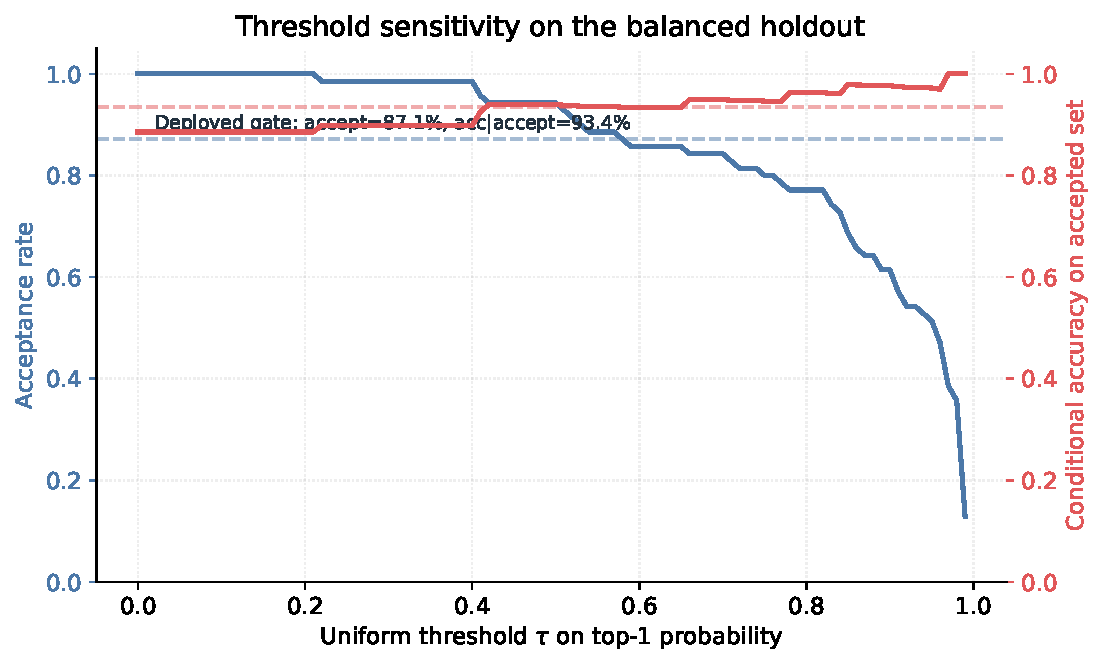
\includegraphics[width=0.92\linewidth]{figures/generated/threshold_sweep.pdf}
\caption{Threshold sensitivity on the balanced holdout under a uniform
threshold $\tau$ on $\bar{p}(\hat{y}\mid x)$. The dashed lines mark
the deployed (per-class) gate operating point.}
\label{fig:threshold-sweep}
\end{figure}

\begin{figure}[H]
\centering
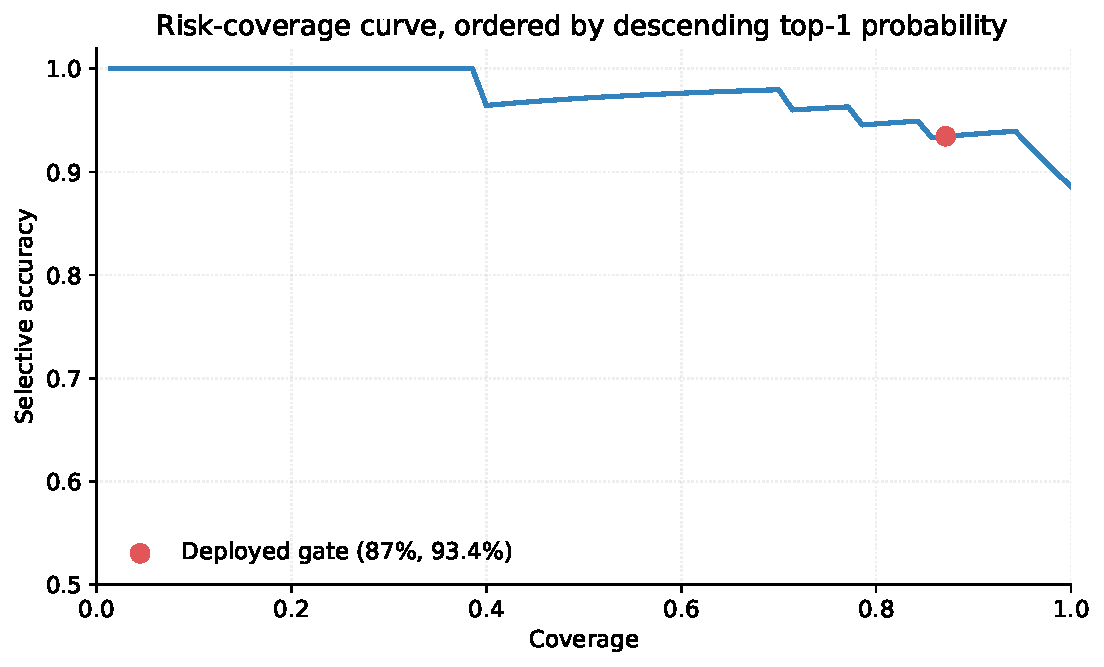
\includegraphics[width=0.92\linewidth]{figures/generated/risk_coverage.pdf}
\caption{Risk-coverage curve obtained by ordering holdout predictions by
descending top-1 probability. The red marker shows the operating point
of the deployed per-class gate.}
\label{fig:risk-coverage}
\end{figure}

\begin{table}[H]
\centering
\caption{Selective top-1 accuracy at fixed coverage levels on the
balanced holdout, computed by ordering predictions by descending top-1
probability.}
\label{tab:selective-acc}
\begin{tabular}{lrr}
\toprule
Coverage & Accepted images & Selective top-1 accuracy \\
\midrule
50\% & 35 & 97.14\% \\
70\% & 49 & 97.96\% \\
85\% & 60 & 93.33\% \\
100\% & 70 & 88.57\% \\
\bottomrule
\end{tabular}

\end{table}

\subsubsection*{Paired comparison of v3 and v4.}

To test whether the v4 retrain produces a statistically distinguishable
improvement over the prior v3 checkpoint on the same holdout, we
performed a McNemar paired test (Table~\ref{tab:mcnemar}). Of the 70
holdout images, both checkpoints agree on 64 (58 both correct, 6 both
incorrect); the v4 retrain is uniquely correct on 4 images and v3 is
uniquely correct on 2. The continuity-corrected
$\chi^2_{\mathrm{1\,df}}$ statistic is $0.167$ (asymptotic two-sided
$p=0.683$; exact binomial two-sided $p=0.688$), which we report
explicitly: the +2.86~percentage-point improvement in top-1 accuracy
from v3 (85.71\%) to v4 (88.57\%) is not statistically significant at
$n=70$. We retain the v4 checkpoint because of (i) the parallel split
hygiene that motivated the retrain (\S\ref{sec:data}) and (ii) the
detector and supervision changes that depend on the same
post-rebuild artifacts.

\begin{table}[H]
\centering
\caption{McNemar paired test comparing v3 and v4 ResNet-50 checkpoints
on the shared 70-image holdout.}
\label{tab:mcnemar}
\begin{tabular}{lr}
\toprule
Quantity & Value \\
\midrule
Holdout size $n$ & 70 \\
Both correct ($n_{11}$) & 58 \\
Only v3 correct ($n_{10} \equiv b$) & 2 \\
Only v4 correct ($n_{01} \equiv c$) & 4 \\
Both incorrect ($n_{00}$) & 6 \\
v3 top-1 accuracy & 85.71\% \\
v4 top-1 accuracy & 88.57\% \\
McNemar $\chi^2$ (continuity-corrected, 1 df) & 0.167 \\
$\chi^2$ asymptotic two-sided $p$ & 0.683 \\
Exact binomial two-sided $p$ & 0.688 \\
\bottomrule
\end{tabular}

\end{table}

\subsection{RF-DETR Grounding-Detector Evaluation}
\label{sec:results-detector}

The grounding detector is an RF-DETR Small instance fine-tuned on a
COCO-style dataset of 753 training images and 322 validation images,
containing 19{,}487 training and 8{,}582 validation instance
annotations across the six-part vocabulary defined in
\S\ref{sec:system}. Training uses 100 epochs at resolution 560 with
batch size 8 and gradient accumulation factor 2 (effective batch 16),
encoder learning rate $1.5\times 10^{-4}$, decoder learning rate
$1\times 10^{-4}$, weight decay $1\times 10^{-4}$, cosine schedule
with five warmup epochs, drop-path $0.1$, and EMA enabled.

Final-epoch validation metrics are summarized in
Table~\ref{tab:rfdetr-final}. The reported quantities follow the COCO
evaluation protocol~\citep{lin2014cocoeval}: average precision at
intersection-over-union threshold 0.5 ($\mathrm{AP}_{50}$),
$\mathrm{AP}_{75}$, the standard $\mathrm{AP}_{50:95}$ average, and
recall-style $\mathrm{AR}$. Best EMA $\mathrm{mAP}_{50}$ on the
validation split is 0.7723 at epoch 93.

\begin{table}[H]
\centering
\caption{RF-DETR Small validation metrics at the final training epoch.
Class-conditional AP is reported at IoU threshold 0.5; aggregate
quantities follow the COCO evaluation protocol~\citep{lin2014cocoeval}.}
\label{tab:rfdetr-final}
\begin{tabular}{lr}
\toprule
Quantity & Value \\
\midrule
$\mathrm{mAP}_{50}$ & 0.772 \\
$\mathrm{mAP}_{50:95}$ & 0.598 \\
$\mathrm{mAP}_{75}$ & 0.644 \\
$F_1$ & 0.737 \\
Precision & 0.798 \\
Recall & 0.687 \\
$\mathrm{AP}_{50}$ flower & 0.611 \\
$\mathrm{AP}_{50}$ fruit & 0.697 \\
$\mathrm{AP}_{50}$ leaf & 0.590 \\
$\mathrm{AP}_{50}$ root & 0.482 \\
$\mathrm{AP}_{50}$ soil & 0.710 \\
$\mathrm{AP}_{50}$ stem & 0.498 \\
EMA $\mathrm{mAP}_{50}$ (best, epoch 93) & 0.772 \\
\bottomrule
\end{tabular}
\end{table}

The intended runtime use of the detector is constraint generation, not
high-fidelity localization. Per-class detection thresholds
$\theta_p$ given in \S\ref{sec:system} were tuned to favor recall on
parts whose absence is more frequently asserted in free-text reports
than presence (e.g., \emph{root}, $\theta_{\mathrm{root}}=0.30$), and
to suppress false positives on the more visually distinct parts
(\emph{flower}, \emph{fruit}, $\theta=0.50$). A formal on/off ablation
of the grounding constraint, evaluated against the language stage on
the holdout, is identified as future work in
\S\ref{sec:results-pending}.

\subsubsection*{Detector behavior on the disease holdout.}

The metrics in Table~\ref{tab:rfdetr-final} are computed on the
detector's own COCO validation split. To characterize behavior on the
deployment distribution, we additionally ran the deployed detector on
the 70 disease-holdout images and recorded the per-class rate at which
each plant part fires above its runtime threshold $\theta_p$
(Table~\ref{tab:rfdetr-holdout}; visualized in
Figure~\ref{fig:rfdetr-heatmap}). Median single-image inference latency
is 18.4~ms (P95 144.2~ms) on a single RTX~3090. The disease holdout
contains no part-level ground truth, so we report visibility-firing
rates rather than precision and recall.

\begin{table*}[t]
\centering
\caption{Per-disease plant-part detection rates of the deployed
RF-DETR Small checkpoint on the 70 disease-holdout images, using the
runtime thresholds $\theta_p$ of \S\ref{sec:system}. The reported
quantity is the fraction of class images for which the corresponding
part fires at least once above $\theta_p$. ``Mean parts'' is the
average number of distinct visible parts per image.}
\label{tab:rfdetr-holdout}
\begin{tabular}{lrrrrrrrr}
\toprule
Disease & $n$ & Flower & Fruit & Leaf & Root & Soil & Stem & Mean parts \\
\midrule
Drought & 10 & 0\% & 60\% & 100\% & 0\% & 40\% & 90\% & 2.90 \\
Frost & 10 & 60\% & 30\% & 100\% & 0\% & 30\% & 90\% & 3.10 \\
Gray mold & 10 & 30\% & 100\% & 90\% & 0\% & 0\% & 90\% & 3.10 \\
Healthy & 10 & 50\% & 100\% & 100\% & 0\% & 40\% & 80\% & 3.70 \\
Overwatered & 10 & 0\% & 10\% & 90\% & 10\% & 80\% & 70\% & 2.60 \\
Root rot & 10 & 0\% & 0\% & 90\% & 100\% & 20\% & 70\% & 2.80 \\
White mold & 10 & 0\% & 100\% & 100\% & 0\% & 0\% & 20\% & 2.20 \\
\textbf{All classes} & \textbf{70} & \textbf{20\%} & \textbf{57\%} & \textbf{96\%} & \textbf{16\%} & \textbf{30\%} & \textbf{73\%} & \textbf{2.91} \\
\bottomrule
\end{tabular}

\end{table*}

\begin{figure}[H]
\centering
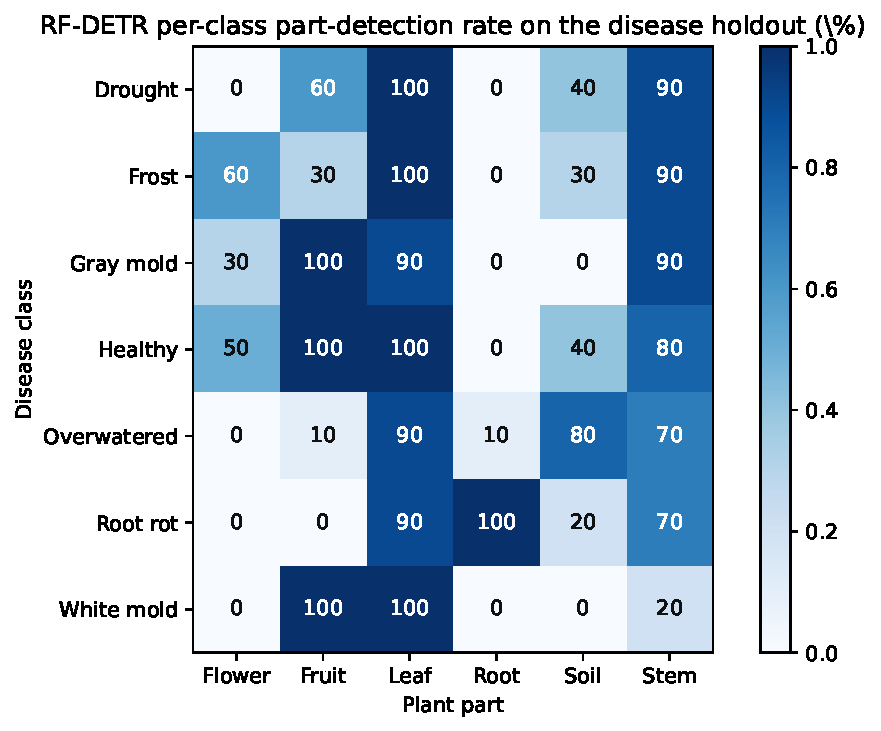
\includegraphics[width=0.92\linewidth]{figures/generated/rfdetr_holdout_heatmap.pdf}
\caption{Per-class plant-part detection rate (\%) of the deployed
RF-DETR Small checkpoint on the disease-holdout images.}
\label{fig:rfdetr-heatmap}
\end{figure}

The pattern is consistent with the deployment intent of the detector:
\emph{leaf} fires on 95.7\% of images across classes, the
\emph{root rot} row fires \emph{root} on 100\% of its images, and
\emph{soil} fires preferentially on \emph{overwatered} (80\%) where
saturated substrate is the dominant visual cue. Detection rates for
\emph{flower} and \emph{root} are otherwise low because those parts are
infrequently visible in the holdout distribution rather than because
the detector is failing.

\subsection{Constrained Dual-Report Pilot}
\label{sec:results-dualreport}

The dual-report pilot is a controlled evaluation of whether the
supervision policy of \S\ref{sec:dualpolicy} produces useful training
targets, rather than a full retraining of the report writer. The
selection routine drew 20 holdout images stratified by class and rule
type. The selection rule counts were 14 close-or-clear-margin
(top-1 matches ground truth) cases of which 2 were close-margin, and 4
top-1-disagrees-with-ground-truth hard cases. Pilot summary statistics
are reported in Table~\ref{tab:dual-report} and visualized in
Figure~\ref{fig:dual-report}.

\begin{table}[H]
\centering
\caption{Statistics for the constrained dual-report pilot
(\S\ref{sec:dualpolicy}). Selection rule counts and report-mode counts
are reported separately. ``Self-reported overclaim risk'' is a generator
metadata field that records the model's own coarse self-rating of
overclaim risk per record.}
\label{tab:dual-report}
\begin{tabular}{lr}
\toprule
Focused tight dual-report pilot statistic & Value \\
\midrule
Selected images & 20 \\
Generated records & 36 \\
Hard-case selections & 4 \\
Close-margin selections & 2 \\
Standard reports & 20 \\
Standard variants & 14 \\
Ambiguous reports & 2 \\
Self-reported low overclaim risk & 28 \\
Self-reported medium overclaim risk & 8 \\
Fallback reports & 0 \\
\bottomrule
\end{tabular}

\end{table}

\begin{figure}[H]
\centering
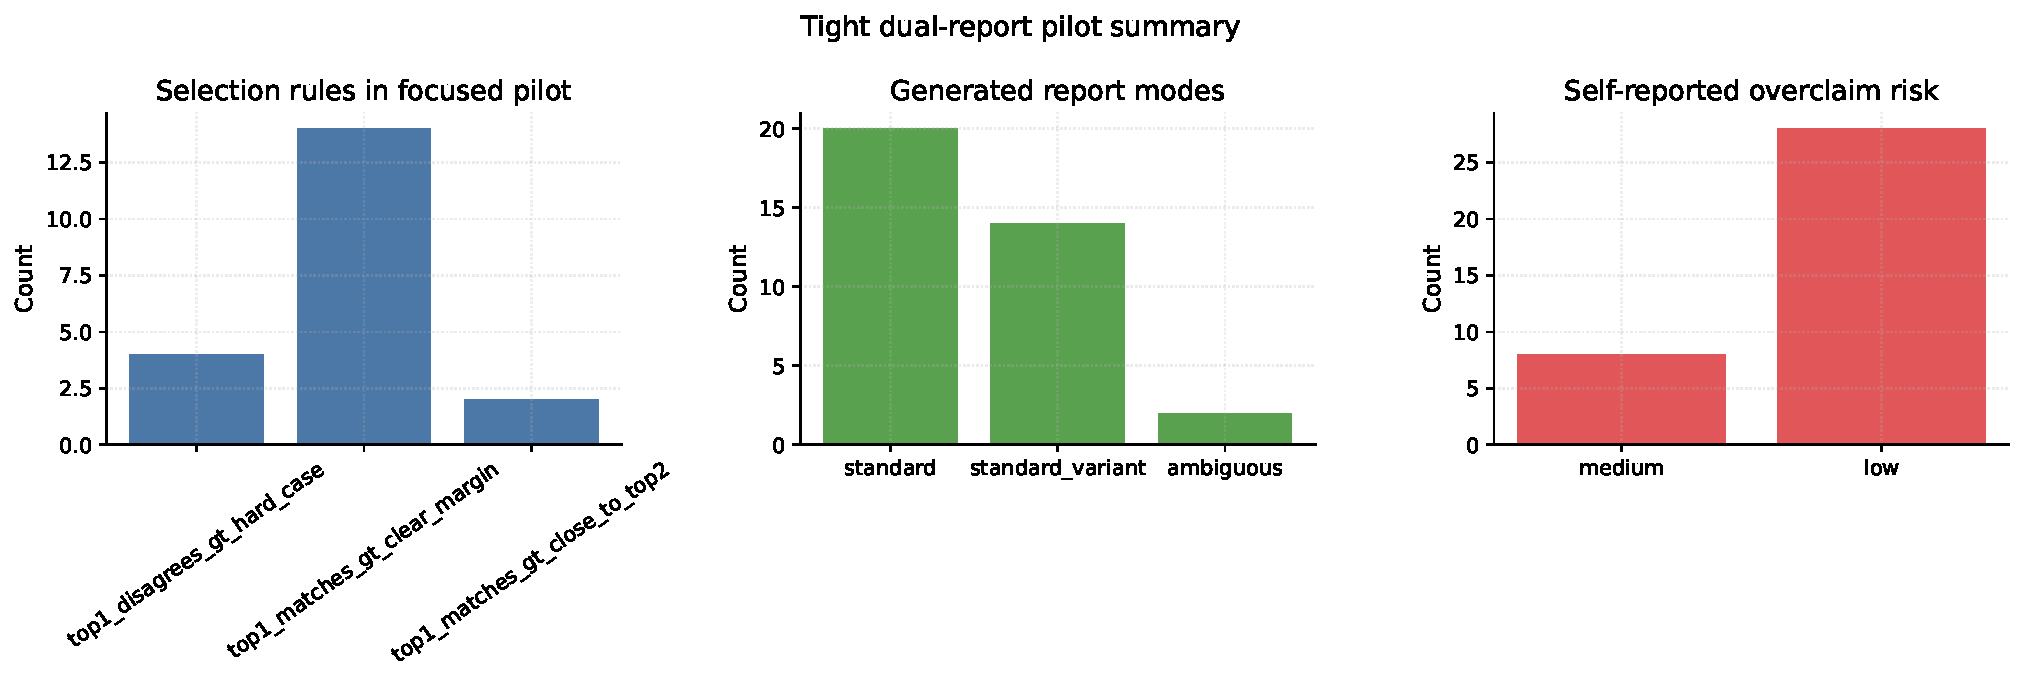
\includegraphics[width=\linewidth]{figures/generated/dual_report_pilot_summary.pdf}
\caption{Constrained dual-report pilot summary. After the policy was
restricted to the pair whitelist of Eq.~\ref{eq:allowed-pairs} and the
margin condition of Eq.~\ref{eq:amb-case-1}--\ref{eq:amb-case-2},
ambiguity reports are rare and concentrated on semantically plausible
disease pairs.}
\label{fig:dual-report}
\end{figure}

The pilot produced 36 records: 20 standard reports, 14 standard
variants, and 2 ambiguity-aware reports. No record required the
fallback generation path. The constrained ambiguity policy filters
out semantically implausible second-rank competitors that arise from
numerical proximity alone; the surviving ambiguity records correspond
to disease pairs that are operationally and visually realistic.

The pilot supports three limited claims:
\begin{enumerate}[leftmargin=1.3em]
\item the dual-report generation pipeline executes end-to-end without
fallback failures;
\item the constrained policy suppresses semantically implausible
ambiguity selections; and
\item the resulting target distribution is sufficient to motivate
full-scale stage-2 regeneration under the same policy.
\end{enumerate}
The pilot does \emph{not} constitute a measurement of post-retraining
explanation quality on the holdout; the deployed MiniGPT-v2 checkpoint
predates the constrained policy.

\subsection{Pending Experiments}
\label{sec:results-pending}

Several experiments are deliberately deferred and are not reported in
this manuscript:

\begin{enumerate}[leftmargin=1.3em]
\item \textbf{Stage-2 regeneration at scale.} The current stage-2
training annotations do not yet encode the constrained policy of
\S\ref{sec:dualpolicy} on the full augmented training set.
\item \textbf{MiniGPT-v2 retraining.} The deployed checkpoint predates
the constrained policy and the holdout carve. A retrained checkpoint is
required before any post-policy explanation claim can be supported.
\item \textbf{Holdout explanation evaluation.} No post-regeneration
explanation rubric has been applied to the retrained checkpoint.
\item \textbf{Grounding ablation.} An on/off ablation of the RF-DETR
visibility constraint, evaluated against the language stage on the
holdout, is planned but not executed.
\end{enumerate}

These items separate a current-state technical report (this paper) from
a finished end-to-end benchmark.
